\section{JSDoc}

Tan importante como el código es la documentación del mismo, JSDoc\footnote{Url del proyecto https://github.com/jsdoc3/jsdoc} es una herramienta inspirada en Javadoc\footnote{http://es.wikipedia.org/wiki/Javadoc} pero pensada para Javascripts. 

Mediante una conjunto de etiquetas (@class, @function, etc) introducidas como comentarios del código fuente,  se generará la documentación en formato HTML\footnote{Por lo general, se genera HTML pero permite otros formatos como RTF.}. Todos los desarrolladores que alguna vez hemos programado en Java y generado documentación de nuestro código, en JavaDoc, estamos familiarizados con el mecanismo de etiquetas, por lo que resulta muy intuitivo la elaboración de la documentación. 

En la figura \ref{fig:codigoconjsdoc} se puede ver un ejemplo de uso de las etiquetas en el código fuente. En concreto de una clase PubSub del propio proyecto MindMapJS. Se puede observar claramente, como se usan etiquetas como @author, @versión, @constrcutor, @class, etc ...  

\begin{figure}[htbp]
\centering
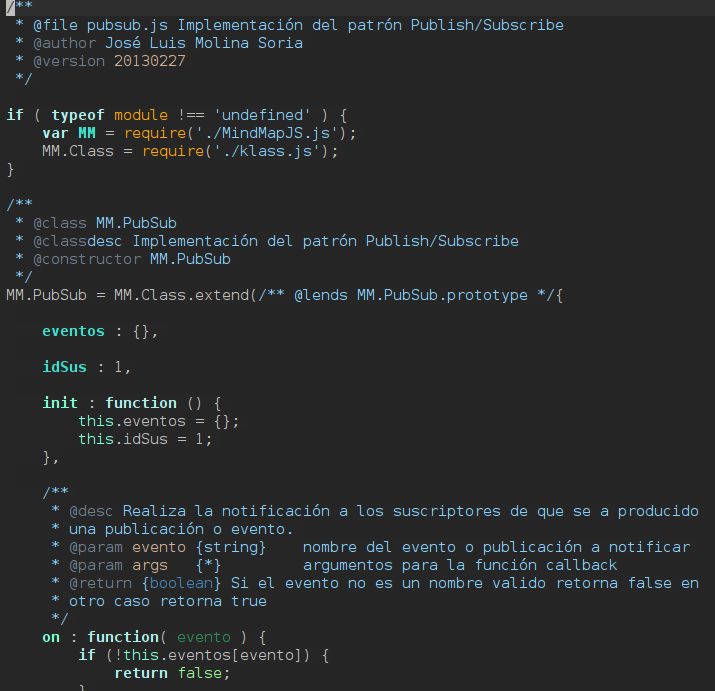
\includegraphics[width=0.7\textwidth]{imagenes/codigoconjsdoc}
\caption{Ejemplo de código fuente documentado con JSDoc}
\label{fig:codigoconjsdoc}
\end{figure}


En la figura \ref{fig:jsdoc} tenemos el resultado de compilar el código fuente con JSDoc. El resultado es un HTML que podemos retocar y configurar, permitiendo tener una Wiki, vistosa y funcional, de la documentación de nuestro código fuente.

\begin{figure}[htbp]
\centering
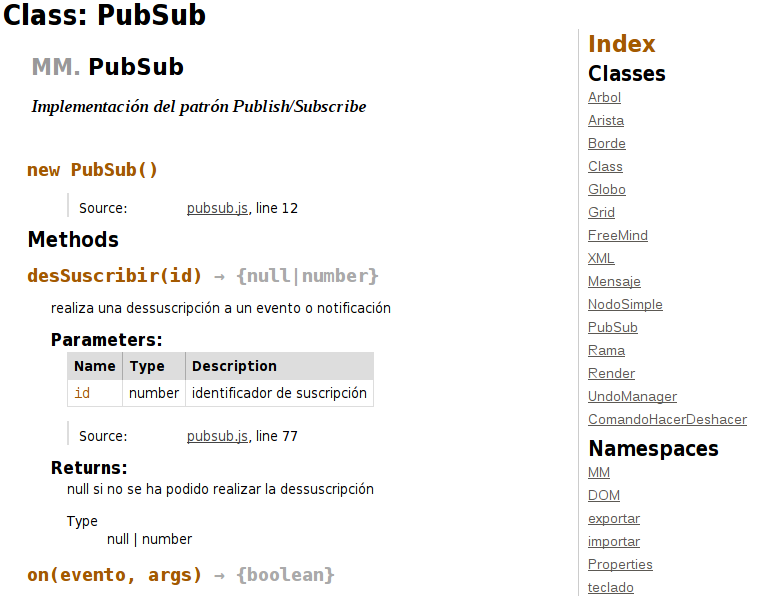
\includegraphics[width=0.7\textwidth]{imagenes/jsdoc}
\caption{Página generada por JSDoc}
\label{fig:jsdoc}
\end{figure}
